\documentclass[10pt, letterpaper]{paper}
\usepackage[margin=0.5in]{geometry}
\usepackage{graphicx}
\usepackage{amsmath}
\usepackage{amssymb}
\usepackage{mathrsfs}
\usepackage{listings}
\usepackage{float}

\title{ Problem Set Five}
\author{ Timothy Schwieg }
\date{ October 11 2017 }

\begin{document}

\maketitle

\section*{Design Document}
This Code should be able to take some input values for $\bar{y}, p, \tau$ and initialization methods for a Newton Method.
It should return the Method of Moments estimators for $pi_0$ and $\lambda$. It will go through this by Iterating Newton steps on the system described by the two moment conditions given in the Problem Ste
Before any steps are taken, the function will parse the input, checking to see that they are valid, and then checks to ensure that the initialiations for Newton's Method are feasible. It will then run Newton steps, stopping after 25 iterations if convergence is not reached, and will check the answer for feasibility. If the value of the estimators is not feasible, it will throw an error and blame the initializations.

\section*{Flow Chart}
\begin{figure}[H]
\centering
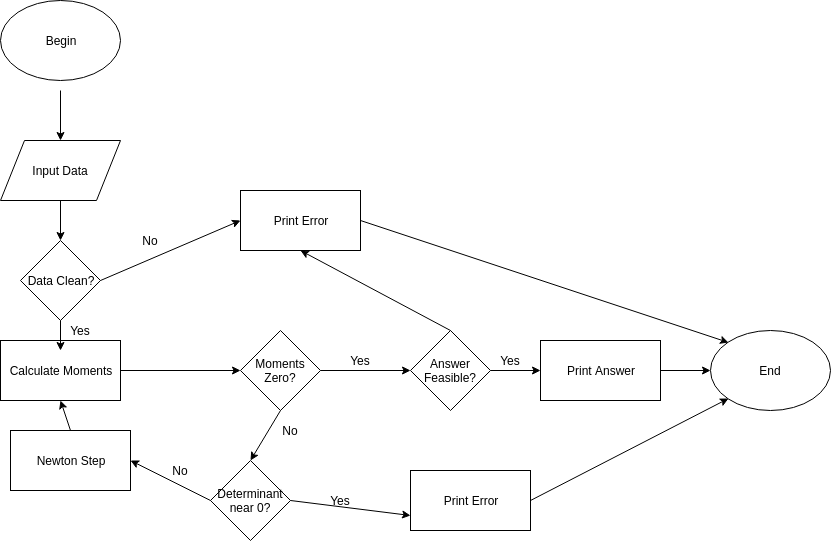
\includegraphics[width=0.8\textwidth]{flowchart.png}
\caption{ Program Flow }
\end{figure}

\section*{Test Data}
Several Test Data with impossible values such as a negative p, $\bar{y}$ or $\tau$ will be tested, as well as impossible initializations such as: $\pi_0 < 0$.
The edge cases to test will be: Small $\bar{y} = .01$ and Large $\bar{y} = 500$ 
We will also try $p=.99$ and $\tau = 1,100$
The last test cases will be where initialization is very far away
$\hat \lambda = 50, \hat \pi_0 = .9$.
As we can see, the code does not break with these absurd cases, but it does not suceed either. The second to last case also highlights the importance of initialization being close for $\hat \lambda$ and the last case shows its irrelevance for $\hat \pi_0$

\begin{lstlisting}[language=sh]
python3 ps5.py -50 .1 3 2 .1
Input error in barY, p, or tau, ITS NOT EVEN WRONG
python3 ps5.py 1 -.1 3 2 .1
Input error in barY, p, or tau, ITS NOT EVEN WRONG
python3 ps5.py 1 .1 -6 2 .1
Input error in barY, p, or tau, ITS NOT EVEN WRONG
python3 ps5.py .01 .1 3 2 .1
Input led to Matrix with determinant close to zero. You've gone off the reservation
ps5.py 500 .1 3 2 .1
Input error in barY, p, or tau, ITS NOT EVEN WRONG
ps5.py 1 .99 3 2 .1
Input led to Matrix with determinant close to zero. You've gone off the reservation
ps5.py 1 .1 1100 2 .1
Input led to Matrix with determinant close to zero. You've gone off the reservation
ps5.py 1 .1 3 50 .1
Convergence reached, but converged to impossible answer. Initialization problem.
[[  1.00000000e-01]
 [ -2.49045000e+03]]
ps5.py 1 .1 3 2 .99
Reached Convergence with hat pi_0 = 0.0690532611049 and hat lambda = 1.13522746211
\end{lstlisting}


\section*{Code}  
Running the code we reach the result: 

\begin{lstlisting}[language=sh]
ps5.py 1 .1 3 2 .1
Reached Convergence with hat pi_0 = 0.0690532611049 and hat lambda = 1.13522746211
\end{lstlisting}


\lstinputlisting[language=python,basicstyle=\tiny]{ps5.py}



\end{document}